% Created 2020-10-07 Wed 09:02
% Intended LaTeX compiler: pdflatex
\documentclass[presentation]{beamer}
\usepackage[utf8]{inputenc}
\usepackage[T1]{fontenc}
\usepackage{graphicx}
\usepackage{grffile}
\usepackage{longtable}
\usepackage{wrapfig}
\usepackage{rotating}
\usepackage[normalem]{ulem}
\usepackage{amsmath}
\usepackage{textcomp}
\usepackage{amssymb}
\usepackage{capt-of}
\usepackage{hyperref}
\usetheme{Luebeck}
\author{Abraham Raji}
\date{October 2, 2020}
\title{What the FOSS!}
\hypersetup{
 pdfauthor={Abraham Raji},
 pdftitle={What the FOSS!},
 pdfkeywords={foss},
 pdfsubject={FOSS as of 2020},
 pdfcreator={Emacs 27.1 (Org mode 9.4)}, 
 pdflang={English}}
\begin{document}

\maketitle
\section*{Introduction}
\label{sec:org75dc288}
\begin{frame}[label={sec:org8774129}]{Hello :)}
\begin{itemize}
\item My name is \href{https://abrahamraji.in}{Abraham Raji}
\item I'm known online as \href{mailto:avronr@tuta.io}{avronr}.
\item Software pays my bills.
\item Web. Cloud. Servers.
\item I am a man with a certain level of appreciation for old things.
\end{itemize}
\begin{block}{Ground Rules}
\begin{itemize}
\item Feel free to interupt me.
They call it seeking knowledge for a reason.
\item No doubts are stupid. People who think otherwise are stupid.
\item Regardless of whether you agree with me or disagree with me it is important you understand me.
\end{itemize}
\end{block}
\end{frame}
\section*{Birth}
\label{sec:orgf21c517}
\begin{frame}[label={sec:orgc546918}]{But does FOSS make sense?}
\begin{columns}
\begin{column}{0.6\columnwidth}
\begin{example}[Something you own]
\begin{center}
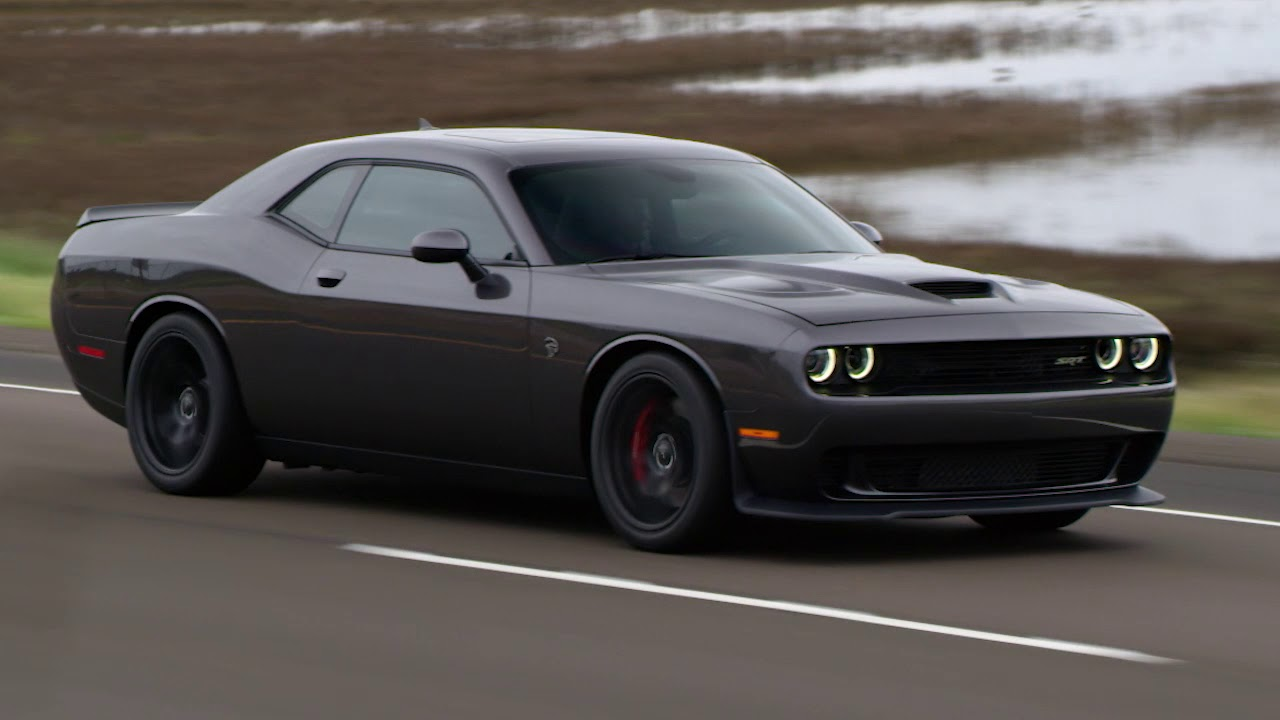
\includegraphics[width=.9\linewidth]{//home/avronr/Code/presentations/what-the-foss/dodge.jpg}
\end{center}
\end{example}
\end{column}
\end{columns}
\end{frame}
\begin{frame}[label={sec:org1426e28}]{But does FOSS make sense?}
\begin{columns}
\begin{column}{0.6\columnwidth}
\begin{example}[Under the Hood]
\begin{center}
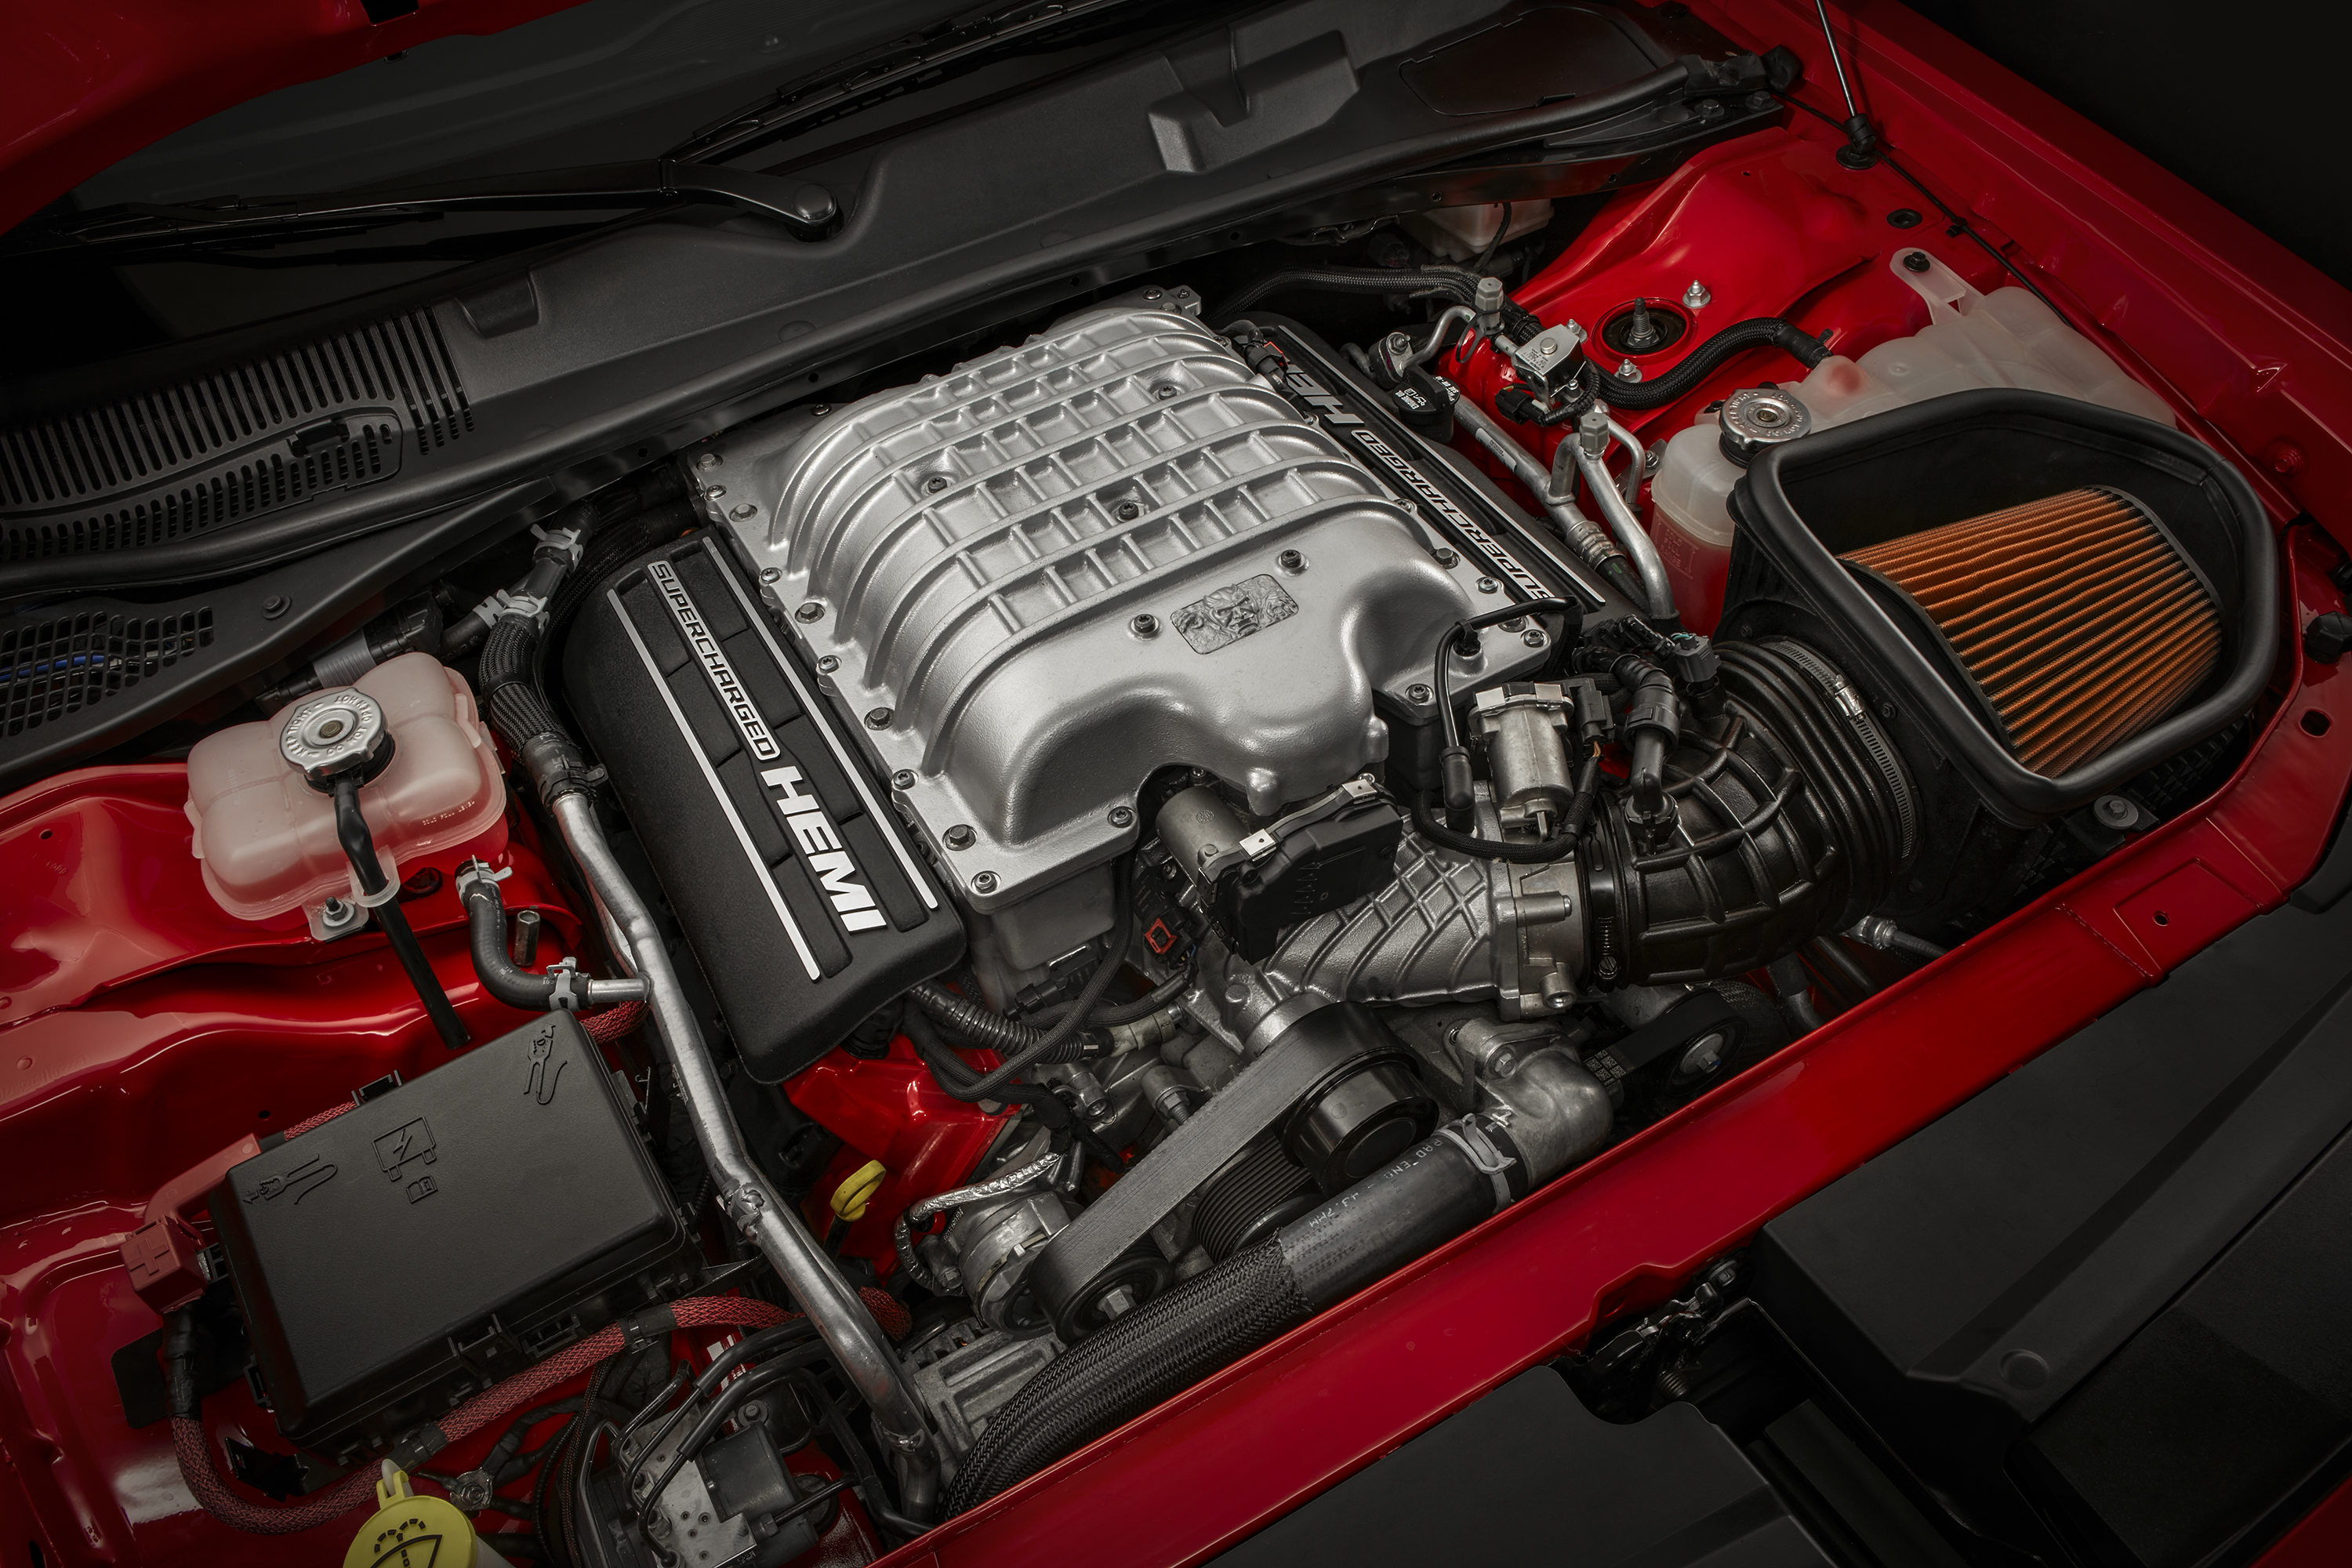
\includegraphics[width=.9\linewidth]{//home/avronr/Code/presentations/what-the-foss/dodge-inside.jpg}
\end{center}
\end{example}
\end{column}
\end{columns}
\end{frame}
\begin{frame}[label={sec:orgcbd0c27}]{But does FOSS make sense?}
\begin{block}{Control}
\begin{quote}
If the users don't control the program, the program controls the users. With proprietary software, there is always some entity, the ``owner'' of the program, that controls the program—and through it, exercises power over its users. A nonfree program is a yoke, an instrument of unjust power.

--- Richard Mathew Stallman \href{https://www.gnu.org/philosophy/free-software-even-more-important.html}{Free Software Is Even More Important Now (September 2013)}
\end{quote}
\hfill \(\qed\)
\end{block}
\end{frame}
\begin{frame}[label={sec:org9bc6414}]{MIT AI Lab}
\begin{columns}
\begin{column}{0.6\columnwidth}
\begin{itemize}
\item 1970s
\item Personal Computers didn't exist.
\item Programming is some people just at the universities knew.
\item They took care of their own needs.
\item They led by Richard M. Stallman started the Free Software Foundation
\end{itemize}
\end{column}
\begin{column}{0.4\columnwidth}
\begin{center}
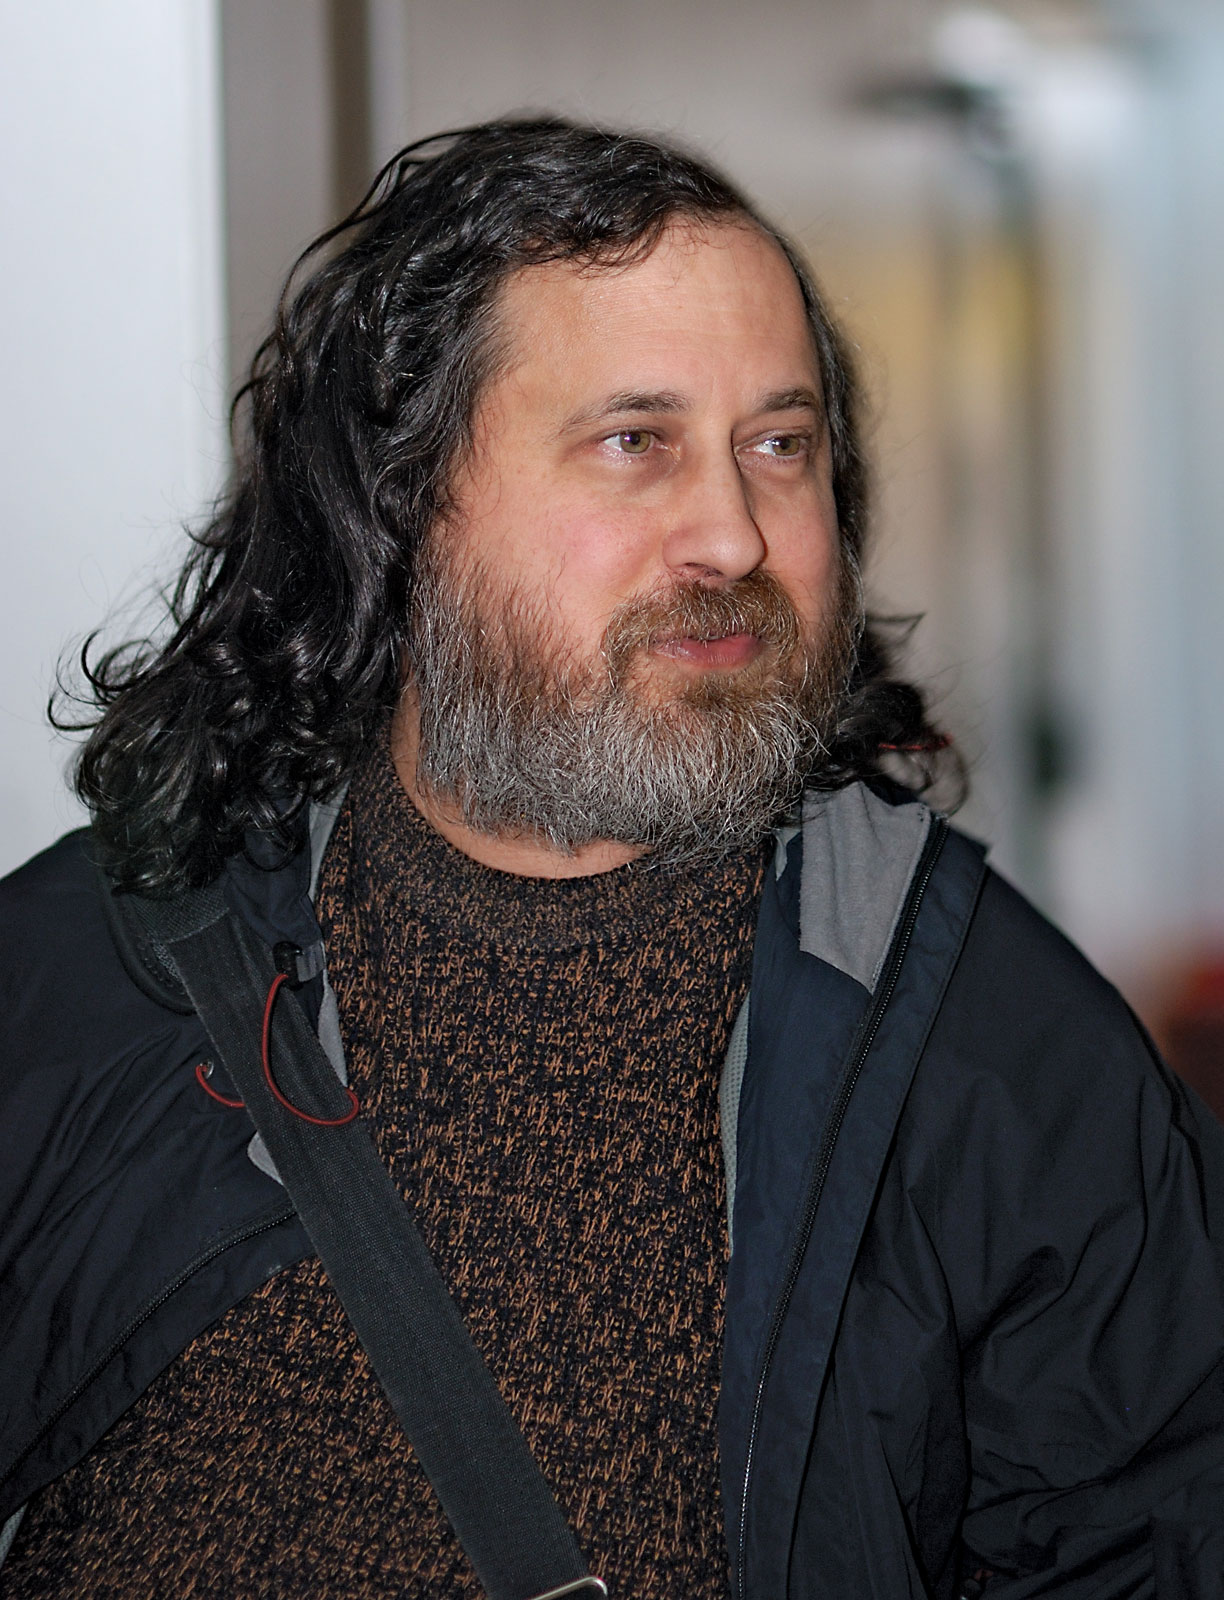
\includegraphics[width=.9\linewidth]{//home/avronr/Code/presentations/what-the-foss/stallman.jpg}
\end{center}
Richard Mathew Stallman
\end{column}
\end{columns}
\end{frame}
\begin{frame}[label={sec:org9566b29}]{Definition}
Free and Open source software is any piece of software that gives it's users the four essential freedoms.
\begin{itemize}
\item The freedom to run the program as you wish, for any purpose (freedom 0).
\item The freedom to study how the program works, and change it so it does your computing as you wish (freedom 1).
\item Access to the source code is a precondition for this. The freedom to redistribute copies so you can help others (freedom 2).
\item The freedom to distribute copies of your modified versions to others (freedom 3). By doing this you can give the whole community a chance to benefit from your changes. Access to the source code is a precondition for this.
\end{itemize}
\end{frame}
\begin{frame}[label={sec:orgdc3b4dd}]{Free Software succeeded because}
\begin{itemize}
\item Users would rather have software that they were able to fix themselves
\item Users would rather use software that they can trust
\item Developers now received suggestions and help from skilled users so their work was easier
\item With more people looking into the software bugs were found and resolved faster.
\end{itemize}
\end{frame}
\begin{frame}[label={sec:orge08456e}]{GNU GPL and the birth of Open Source}
\begin{columns}
\begin{column}{0.6\columnwidth}
\begin{itemize}
\item The single document that determines whether a piece of software is free software or not is it's Licence.
\item GPL prevented Free Software from being used in proprietary software.
\end{itemize}
\end{column}
\begin{column}{0.4\columnwidth}
\begin{center}
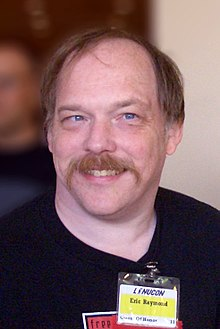
\includegraphics[width=.9\linewidth]{//home/avronr/Code/presentations/what-the-foss/esr.jpg}
\end{center}
Eric S Raymond
\end{column}
\end{columns}
\end{frame}
\begin{frame}[label={sec:org851e145}]{Open Source vs Free Software}
\begin{center}
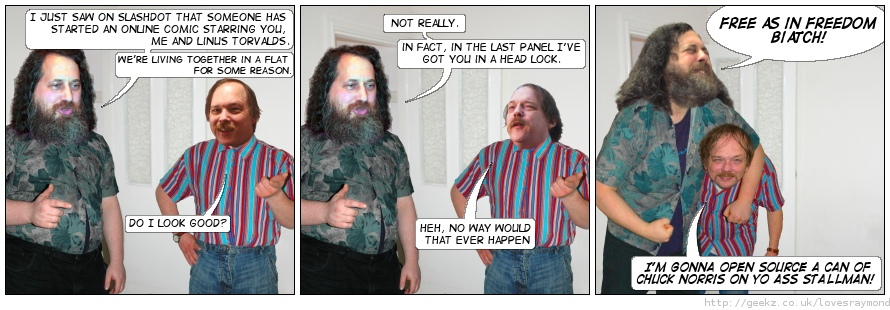
\includegraphics[width=.9\linewidth]{//home/avronr/Code/presentations/what-the-foss/ep000.jpg}
\end{center}
\end{frame}

\section*{Free Software in Real Life}
\label{sec:org847b9f9}
\begin{frame}[label={sec:org998676b}]{Can a Company make money out of Free Software?}
\begin{itemize}
\item Short Answer: Yes
\item Real life examples: Redhat, Suse, Canonical, Gitlab and More
\item Most of the revenue for software companies comes from Corporates
\begin{itemize}
\item Corporates value reliability.
\end{itemize}
\end{itemize}

\begin{center}
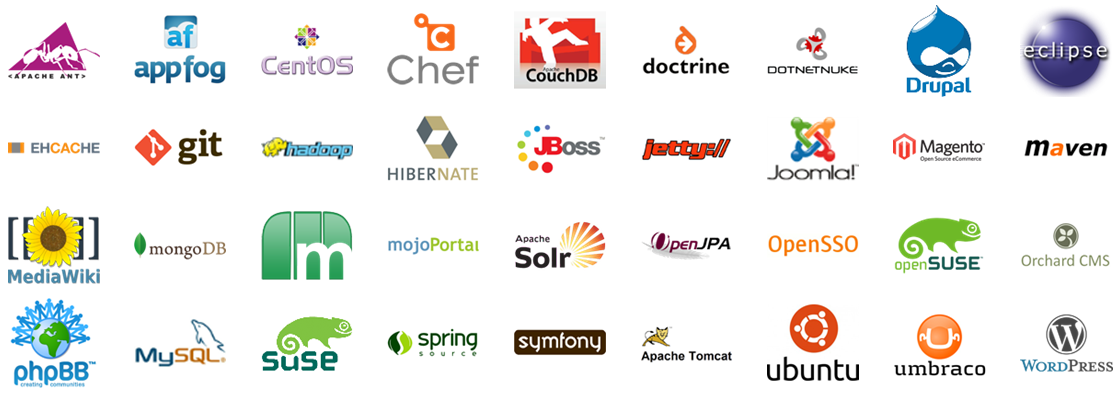
\includegraphics[width=.9\linewidth]{//home/avronr/Code/presentations/what-the-foss/comp.png}
\end{center}
\end{frame}
\begin{frame}[label={sec:orgc2b8aa1}]{Can an individual make a living out of Free Software?}
\begin{itemize}
\item Short Answer: Yes.
\item You can work at the above mentioned companies.
\item You can provide support for free software.
\item You can work on or created projects supported by a community or corporate.
\end{itemize}
\end{frame}
\section*{Free Software in India}
\label{sec:org249a78a}
\begin{frame}[label={sec:org2ba28a5},fragile]{Free Software Projects and Communities based in India.}
 \begin{itemize}
\item Free Software Community of India (FSCI) \texttt{fsci.in}
\item Swathanthra Malayalam Computing \texttt{smc.org.in}
\item Mozilla Kerala \texttt{mozillakerala.com}
\item Leapcode \texttt{leapcode.io}
\item Various Free Software and Linux User Groups
\item Student Developers Society \texttt{studevsoc.in}
\end{itemize}
\end{frame}
\begin{frame}[label={sec:org4351c6d}]{Questions}
\begin{block}{Ask Away !}
\end{block}
\end{frame}
\begin{frame}[label={sec:org6720cb7}]{Get in touch with me}
\begin{itemize}
\item Gitlab: avron
\item Mail: avronr@tuta.io
\end{itemize}
\end{frame}
\end{document}
